\subsection{Entry indicator}

\begin{figure}[htbp]
   \centering
   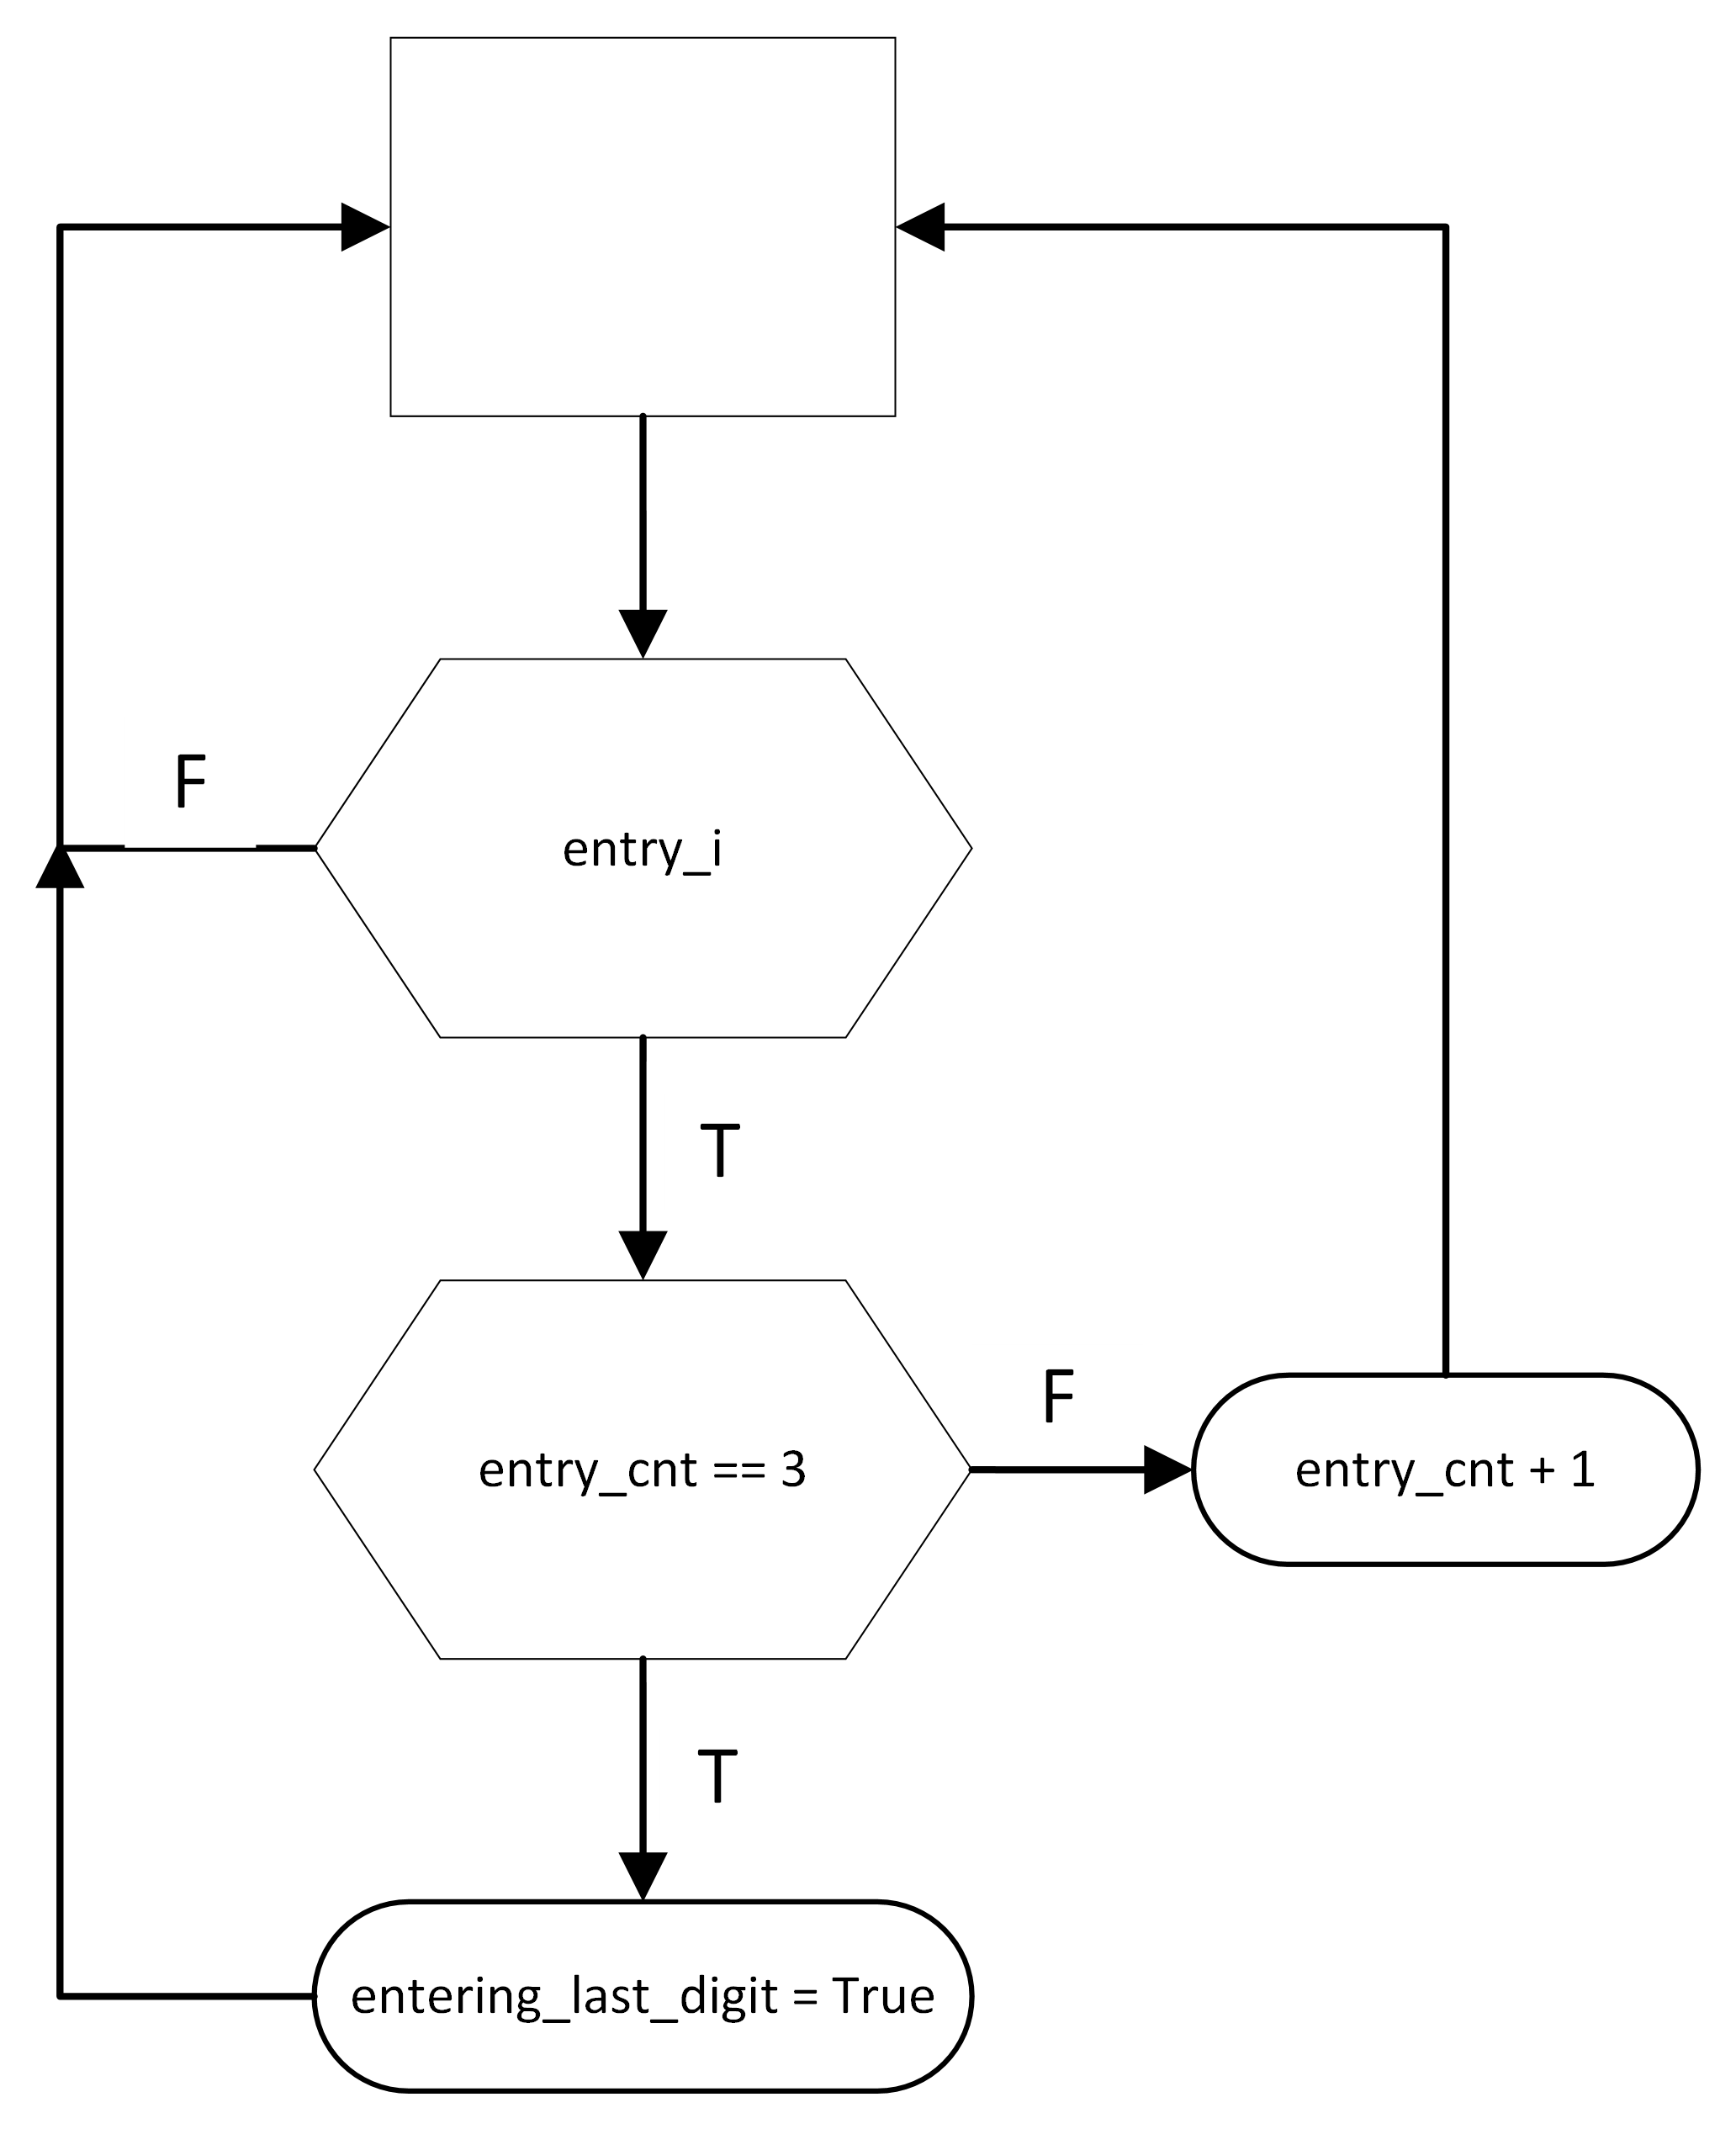
\includegraphics[width=0.85\textwidth]{entry_indicator_asm.png}
   \caption{ASM chart of the entry indicator module.}
   \label{fig:entry_indicator_asm}
\end{figure}

\begin{minted}[
   fontsize=\footnotesize,
   linenos,
   breaklines,
]{verilog}
module entry_indicator (
   input clk_i,
   input rst_ni,
   input entry_i,
   output entering_last_digit_o
);

reg [2:0] state_d, state_q;
parameter EnteringLastDigit = 3'd3;

assign entering_last_digit_o = state_q == EnteringLastDigit;

always @(posedge clk_i, negedge rst_ni)
   if (~rst_ni)
      state_q <= 3'd0;
   else
      state_q <= state_d;

always @(state_q, entry_i) begin
   state_d = state_q;  // default assignment next state is present state
   if (entry_i)
      if (state_d == EnteringLastDigit)
         state_d = EnteringLastDigit;
      else
         state_d = state_d + 1'b1;
end

endmodule
\end{minted}

\begin{minted}[
   fontsize=\footnotesize,
   linenos,
   breaklines,
]{verilog}
module entry_indicator_tb;

// Inputs
reg clk;
reg rst_n;
reg entry_i;

// Outputs
wire entering_last_digit_o;

entry_indicator DUT (
   .clk_i(clk),
   .rst_ni(rst_n),
   .entry_i(entry_i),
   .entering_last_digit_o(entering_last_digit_o)
);

// Create a 50Mhz clock
always #10 clk = !clk;  // every ten nanoseconds invert

initial begin
   clk = 1'b0;
   rst_n = 1'b0;
   entry_i = 1'b0;
end

initial begin
   #20 rst_n = 1'b1;  // release reset

   repeat (6) begin
      @(posedge clk);
      entry_i = 1'b1;
      @(posedge clk);
      entry_i = 1'b0;
   end

   #40;

   $finish;
end

endmodule
\end{minted}

\begin{figure}[htbp]
   \centerline{
   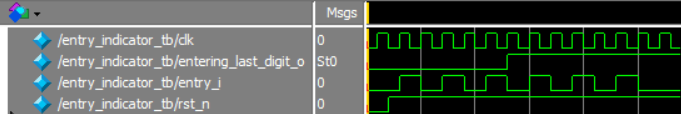
\includegraphics[width=\paperwidth]{entry_indicator_sim.png}}
   \caption{Testbench simulation of the entry indicator module.}
   \label{fig:entry_indicator_sim}
\end{figure}

Fig.~\ref{fig:entry_indicator_sim} shows that the indicator raises entering-last-digit flag signal after entering the third digit (forth digit is the last digit as per the assignment brief).
